\documentclass[a4paper]{article}
\usepackage{geometry}                % See geometry.pdf to learn the layout options. There are lots.
\geometry{letterpaper}                   % ... or a4paper or a5paper or ... 
%\geometry{landscape}                % Activate for for rotated page geometry
%\usepackage[parfill]{parskip}    % Activate to begin paragraphs with an empty line rather than an indent
\usepackage{graphicx}
\usepackage{amssymb}
\usepackage{epstopdf}
\usepackage{multicol}
\usepackage{tikz}
\usetikzlibrary{calc}
\usepackage{mathptmx}
\usepackage{amsmath}

\DeclareGraphicsExtensions{.pdf,.png,.jpg}
\usepackage{wrapfig}

% Spacing stuff
\usepackage[cm]{fullpage}
\addtolength{\voffset}{-1in}
\setlength{\topmargin}{0pt}
\setlength\footskip{0pt}
\setlength{\parskip}{0cm}
\setlength{\parindent}{1em}
\usepackage[compact]{titlesec}
\titlespacing{\section}{0pt}{2ex}{1ex}
\titlespacing{\subsection}{5pt}{1ex}{2ex}
\titlespacing{\subsubsection}{0pt}{0.5ex}{0ex}

\title{Packing Game - Parts A and B}
\author{
Donnie Smith (donnie.smith@gatech.edu) \\
Kyle Harrigan (kwharrigan@gmail.com) 
}	
\date{September 6, 2012}                                           % Activate to display a given date or no date

\begin{document}
\begingroup
\let\center\flushleft
\let\endcenter\endflushleft
\maketitle
\endgroup

\begin{tikzpicture}[remember picture,overlay]
  \node[anchor=north east,inner sep=0pt] at ($(current page.north east)-(1cm,0cm)$) {
     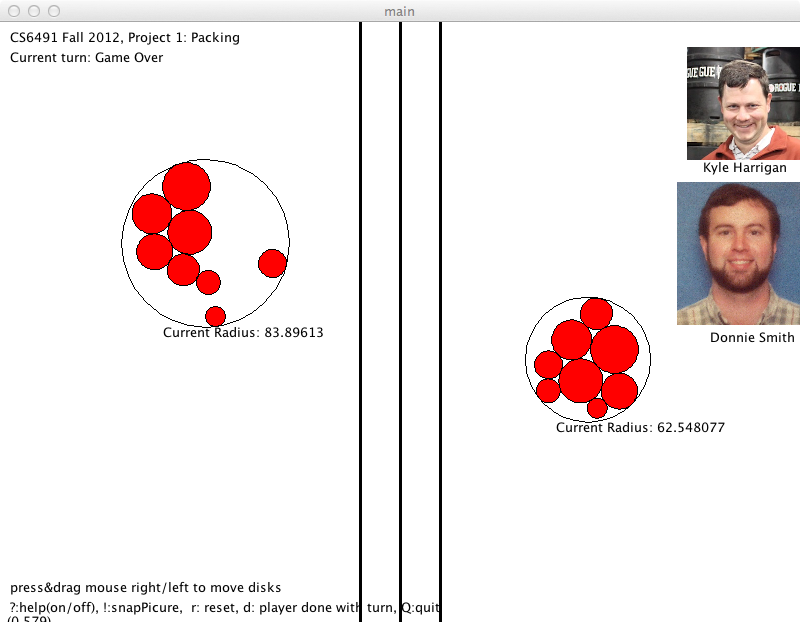
\includegraphics[width=300px,height=180px]{main/data/screenshot.png}

  };
\end{tikzpicture}


 \subsection*{Problem Statement}
  
Implement an application which allows two human players to compete in an intense battle of disk packing.  The goal is for players to pack the disks as tightly as possible, resulting in the smallest enclosing sphere.  The program must calculate the minimal enclosing sphere, assign a score to each user, and declare a winner.  
 
 \subsection*{Completed Features}
 \begin{multicols}{2}
 \begin{itemize}
 \setlength\multicolsep{0pt}
\itemsep0em 
\item Read disk count and disk sizes from file
\item Create initial holding area for discs
\item Limit disk movement to appropriate player's side
\item Pairwise and triplet collision detection
\item Bounding circles for pairs and triplets(minimal containing disk)
\item Scoring and basic gameplay
\item Physics-based AI Player 
\end{itemize}
\end{multicols}

 \subsection*{To Be Done}
  \begin{multicols}{2}
 \begin{itemize}
\item Need to improve collision detection-- remove "flipping" and overlap conditions
\item Possibly optimize computation of minimal containing disk
\item AI collision detection improvements
\end{itemize}
\end{multicols}
 
\subsection*{Computing Minimal Containing Disk}
The minimal containing circle was computed by finding the minimal containing circles for all pairs and some triplets of the circles.
The algorithm functions as follows:
\begin{enumerate}
	\item The current best solution is initialized to an impossibly large radius.
	\item For each pair of circles:
	\begin{enumerate}
		\item The minimum containing circle is computed.  If the radius of that circle is smaller than the current best solution:
		\begin{enumerate}
			\item If it contains all circles, then the current best solution is set to that circle.
			\item Otherwise, the minimal containing circle of all triplets that includes the initial pair are considered.  If that circle contains all circles:
			\begin{enumerate}
				\item If the circle is smaller than the current best solution, then the current best solution is set to that circle.
			\end{enumerate}
		\end{enumerate}
	\end{enumerate}
\end{enumerate}

This algorithm is not the most efficient available, but runs in $O(n^4)$ time, which is acceptable for a small number of circles.
The solution to the minimal bounding circle for triplets, which is one of the ten cases of Apollonius' Problem, was adapted from code written by Rasmus Fonseca.
The code was modified to fix a bug in which an invalid solution is found when two of the three circles are vertically aligned.

\subsection*{Physics-Based AI Model}

\subsubsection*{Introduction}

Instead of a graph-based approach, we chose to employ a physics-based approach which models physical disks that move in a 2D plane.  Initially, disks are spread out in a circular pattern, and then a forcing function is applied at each update in an attempt to search for the best solution.  A description of the algorithm steps follows.  

\subsubsection*{Initialization}
Disks are initially spread disks out in a circular pattern

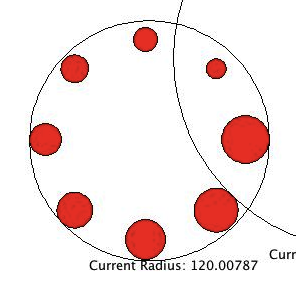
\includegraphics[width=200px,height=180px]{main/data/physics_init_clipped.png}

\subsubsection*{Iterate}

\begin{itemize}
\itemsep0em
\item{At each step, we compute the new the center of gravity.  The center of gravity is moved in order to induce a "shaking" or "shuffling" effect upon the disks}


\begin{align}
     da & = 0.1 \\
      angle & = (angle + da) \\ % TWO_PI; 
      x & = center_x + center_r\times cos(angle) \\
      y & = center_y + center_r\times sin(angle)
\end{align}

\item{For each disk, compute the velocity according to the forcing function (currently a velocity impulse):}

\begin{align}
      dx &= x - cursor.x \\
      dy &= y - cursor.y \\
      center_x &= cursor.x + dx*sq(cursor.r)/20*dt \\
      center_y &= cursor.y + dy*sq(cursor.r)/20*dt
\end{align}
	\begin{itemize}
	\itemsep0em
  \item{Linear in the distance of the disk from the center of gravity}
  \item{Quadratic in the radius of the disk}
  \end{itemize}
\item{Then, sort by increasing radius from the center of gravity}
\begin{itemize}
\itemsep0em
 \item{The purpose of the sort is to be able to detect all collisions with a single pass, as long as we can guarantee that no disk is moved towards the center of gravity as a result of collision detection}
 \end{itemize}
 \item{Finally, compute the minimum bound, compare to the smallest seen minimum bound and if it is smaller record the disk configuration at this minimum value}
 \end{itemize}
  
\subsubsection*{Stopping Condition}
The physics-based model iterates over time.  
\begin{itemize}
\itemsep0em
\item{Currently fixed at 2000 iterations which produces a reasonable solution that beats most humans}
\item{Once the iterations are completed, we reset to configuration to the seen number of minimum disks and display}
\end{itemize}

  
\subsection*{References}
\begin{itemize}
\itemsep0em
	\item http://en.wikipedia.org/wiki/Smallest\_circle\_problem
	\item http://mathworld.wolfram.com/ApolloniusProblem.html
	\item http://www.diku.dk/hjemmesider/ansatte/rfonseca/
	\item For handling multiple collisions (circle intersection problem) http://paulbourke.net/geometry/2circle/
\end{itemize}
\end{document}  
